\subsection*{Use Case Appendix}

\subsubsection*{Concentration Time Traces}
From the output of the simulator, we get the evolution of the abundance of
Cat through time. In Figure~\ref{F0}, we can see the systems with low phosphatase
behave similarly, even though one has five times the amount of kinases
than the other (blue vs red traces). In contrast, the system with high
phosphatase shows markedly less degradation of Cat; where the other
two system degraded around 450 units, this one has only degraded
23. From this whole-system view, it would seem the amount of
phosphatase is more critical than the amount of kinase: based on the
1:1 system, increasing the kinase five fold has little effect, whereas
increasing the phosphatase has a more dramatic effect.

\begin{figure}[h]
  \centering
  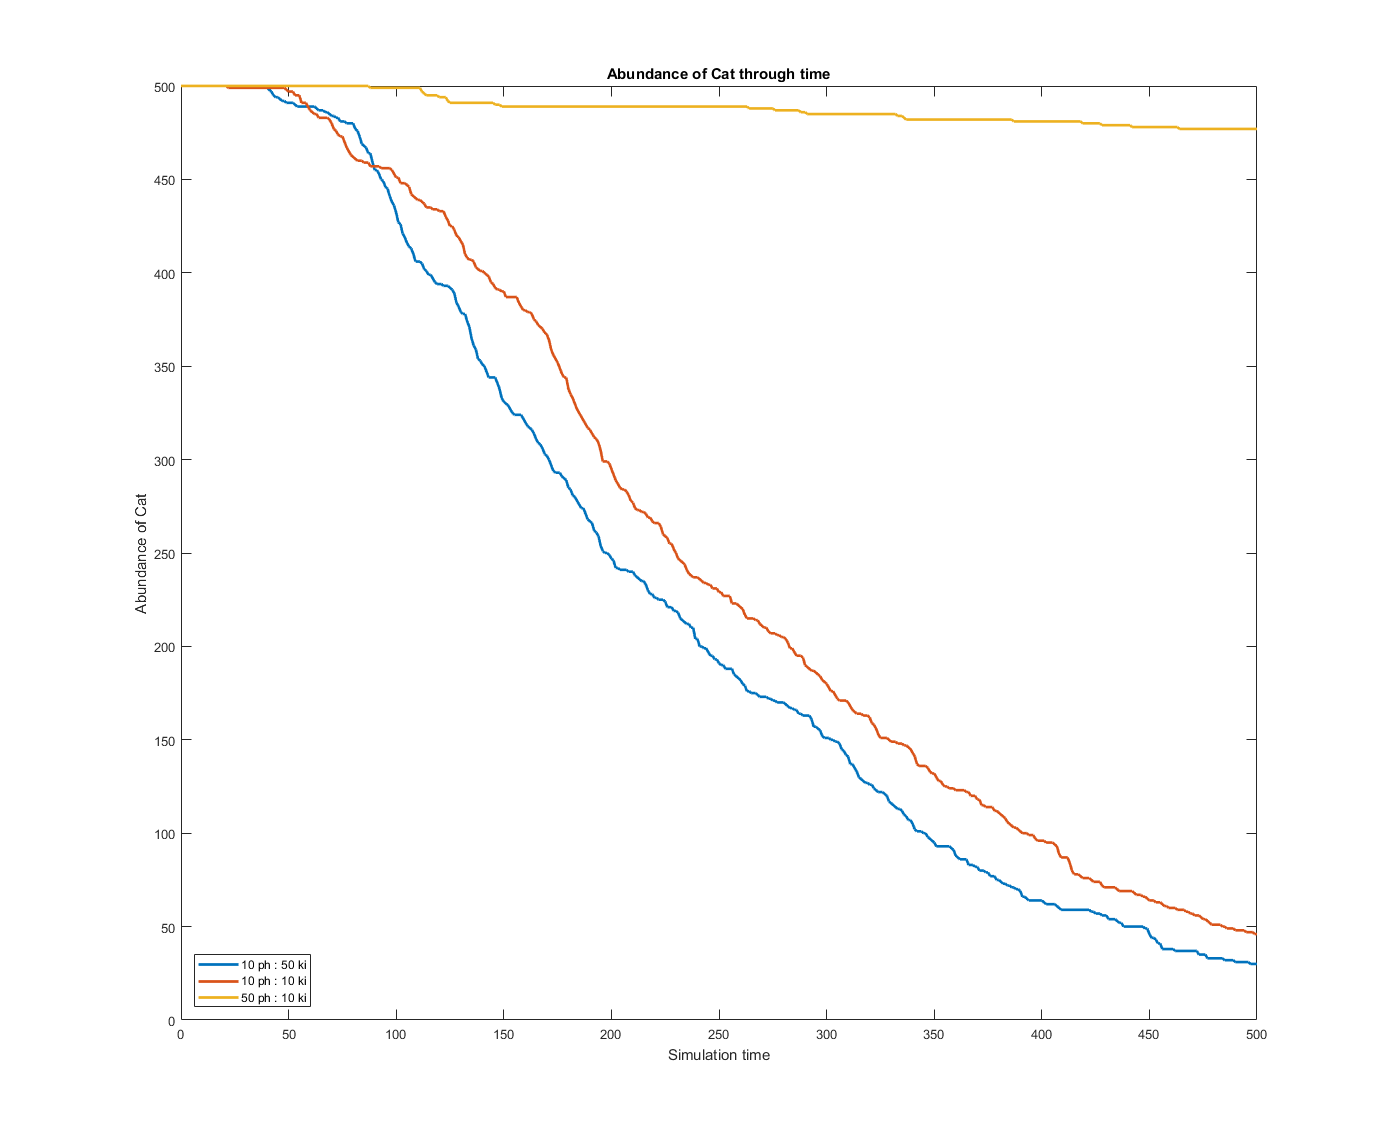
\includegraphics[width=\columnwidth]{wnt/F0_abundance_of_cat_through_time}
  \caption{Tracking the abundance of agent Cat through the
    simulation. At time $T=0$, the agents are introduced, all in
    monomeric form. The simulation was stopped after five hundred
    simulated seconds. In this legend and throughout the figures, ph
    stands for phosphatase, ki stands for kinase, and the agent
    numbers are presented. Thus ``$10$ ph : $50$ ki'' means the system
    with $10$ units of phosphatase and $50$ of kinase.}
  \label{F0}
\end{figure}


\subsubsection{Complex composition: all four on the same component?}

For the final query, we wonder if all four final phosphorylation
events occur on the same complex. Given the short wait time
(Figure~\ref{F2}), one might expect so, but the number of
dephosphorylation events is so large (Figure~\ref{F1}), it could be
well that a substrate is partially modified on one complex,
subsequently modified on another, finalized in yet another. Lacking a
metric by which we can compare complexes for distance, we instead
compare complex compositions as a proxy.

Seeing how overwhelmingly, for each specific modification on a single Cat, the
S45 phosphorylation events happened on complexes of the same Axn and
APC composition as the T41 phosphorylation events, as the S37
phosphorylation events, as the S33 phosphorylation events, we feel
confident in claiming all four steps occurred on the same
complex. This agrees well with the observation that the wait times are
fairly short (Figure~\ref{F2}). We did not see an appreciable
difference for the other parameter regimes.

\begin{figure}[h]
  \centering
  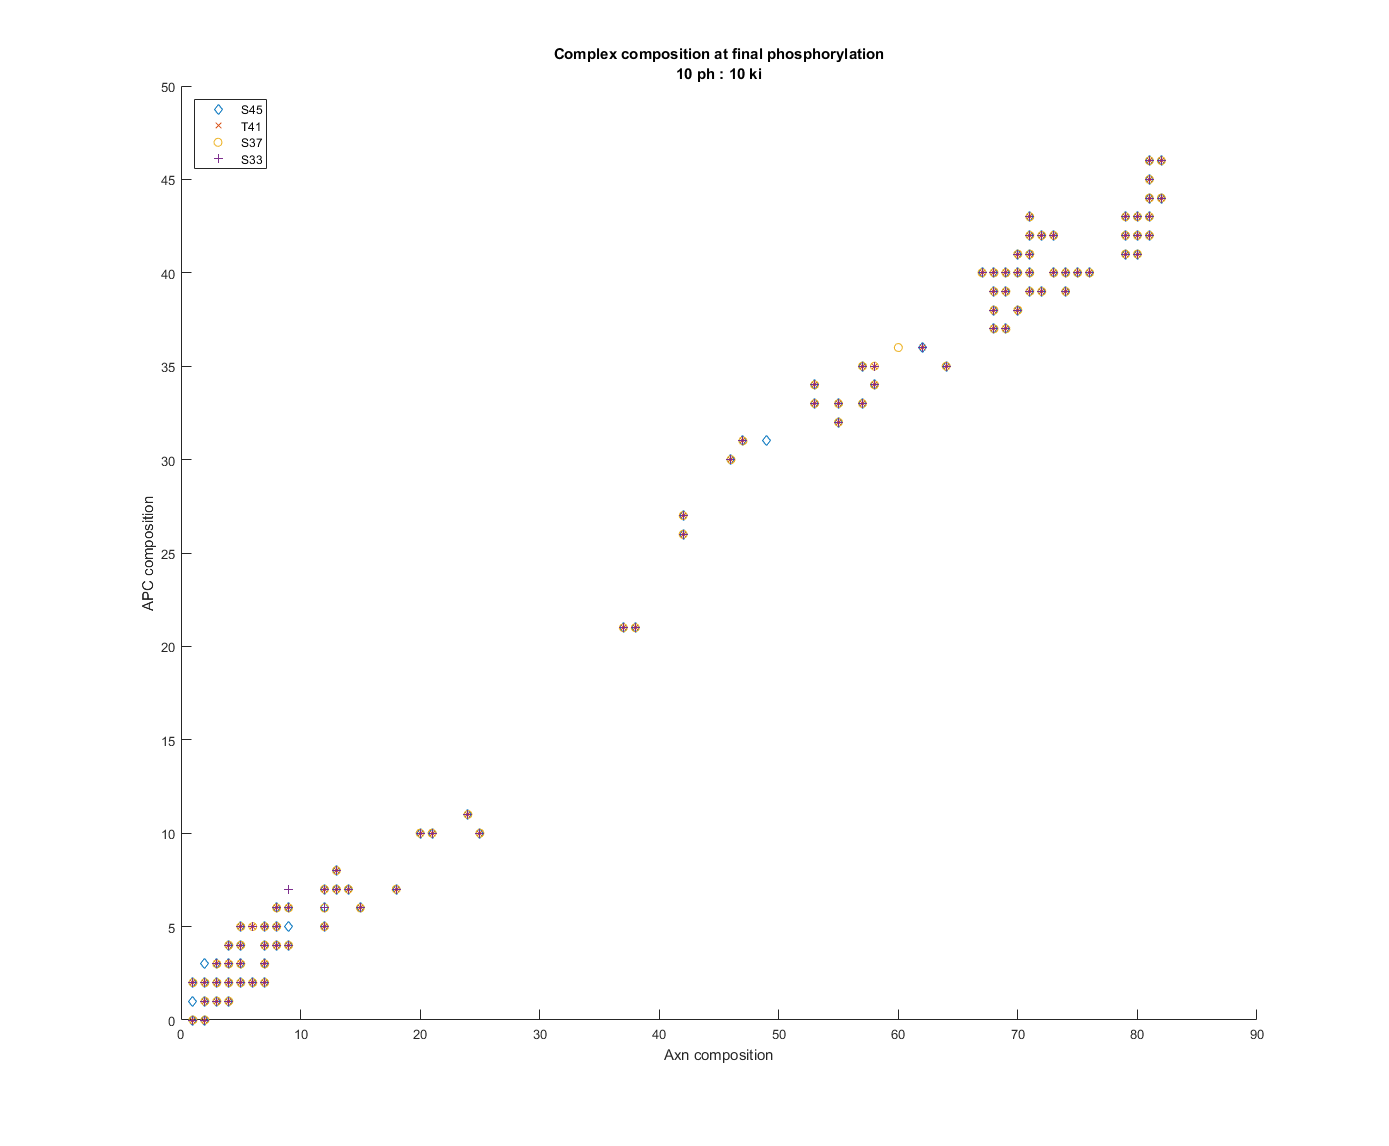
\includegraphics[width=\columnwidth]{wnt/F11_complex_composition_10_10}
  \caption{Complex composition at the time of the last phosphorylation
    for the 1:1 system. All four residues are shown. A diamond
    superposed with a cross superposed with a circle superposed with a
    plus sign indicates all four modifications for a specific copy of
    Cat occurred on a complex of the same composition in terms of Axn
    and APC. We interpret this as having occurred on the exact same
    complex.}
  \label{F11}
\end{figure}